\begin{frame}
\frametitle{RealNVP}
    \begin{itemize}
        \item Stands for ``Real-valued Non-Volume Preserving transformations"
        \item Demonstrate ability to model natural images through sampling,
        log-likelihood evaluation, and latent variable manipulations.
        \item Builds on NICE
        \item Generates sharper images and helps with batch norm and ResNets
    \end{itemize}
    MLE
    \begin{equation*}
        p_X(x) = p_Z(z) \left| det\left(\frac{\partial g(z)}{\partial
                z^T}\right)\right|^{-1}
    \end{equation*}
\end{frame}

\begin{frame}
\frametitle{Change of Variables}
Given an observed variable $x\in X$, a prior probability distribution $p_z$
on latent variable $z\in Z$, and a bijective function $f:X\rightarrow Z$
($g=f^{-1}$)
    \begin{align*}
        p_X(x) &= p_Z(f(x))\left | det \left(\frac{\partial f(x)}{\partial
                x^T}\right)\right|\\
        log(p_X(x)) &= log(p_Z(f(x))) + log\left(\left|def\left( \frac{\partial
                    f(x)}{\partial x^T}\right)\right|\right)
    \end{align*}
We can then draw a sample $z\sim p_Z$ in the latent space and its inverse image.
\end{frame}

\begin{frame}
\frametitle{Computational Graph}
\begin{figure}
    \centering
    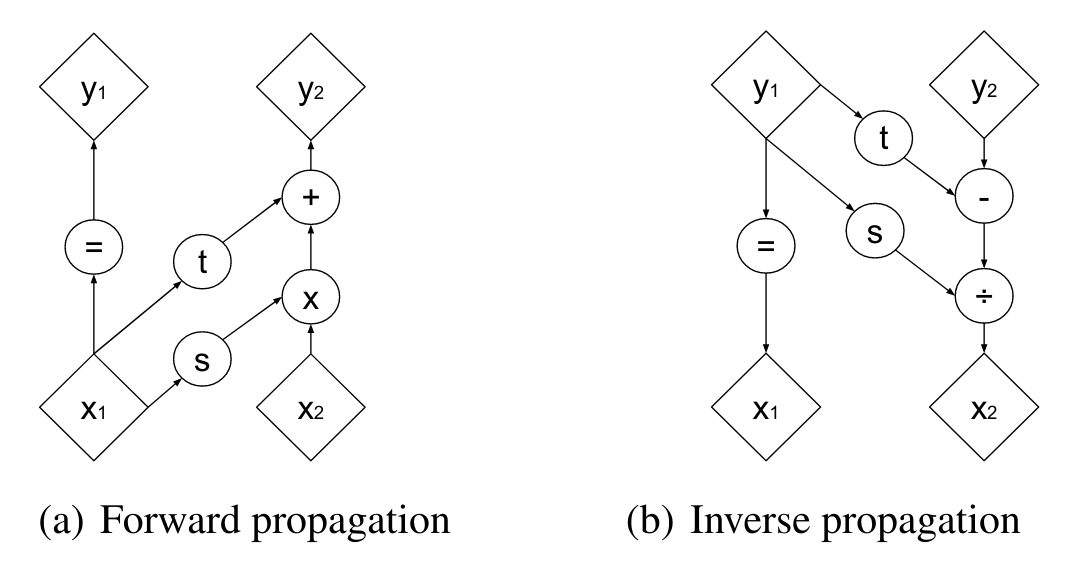
\includegraphics[width=0.8\textwidth]{RealNVPComputationalGraph}
\end{figure}
\end{frame}

\begin{frame}
\frametitle{Bijective Function}
Given a dimensional input $x$ and $d<D$ we can create an affine coupling layer
$y$.
    \begin{align*}
        y_{1:d} &= x_{1:d}\\
        y_{d+1:D} &= x_{d+1:D} \odot exp(s(x_{1:d})) + t(x_{1:d})
    \end{align*}
Here $s$ is for a scalar transform, $t$ is for a translation, and functions are
$R^d \mapsto R^{D-d}$. $\odot$ is the standard element-wise product (Hadamard)

\end{frame}

\begin{frame}
\frametitle{Jacobian}
Exploits that the determinant of a triangular matrix is the product of the
diagonals.
\begin{equation}
\frac{\partial y}{\partial x^T} = \begin{bmatrix} \mathbb{I}_d & 0 \\
        \frac{\partial y_{d+1:D}}{\partial x_{1:d}^T} & diag(exp[s(x_{1:d})])
        \end{bmatrix}
\end{equation}
Hidden layers of $s$ and $t$ can have more features than their input or output
layers.
\end{frame}

\begin{frame}
\frametitle{Summary of Other Properties}
    \begin{itemize}
        \item Uses a squeezing operation to make sampling as efficient as an
        inference model.
        \item Partitioning can be done with a binary mask
        \item $s$ and $t$ are rectified CNNs
        \item Multiscale architecture by using a squeezing operation (divides
                each channel into 2x2xc then reshapes to 1x1x4c $s\times s\times
                c \mapsto \frac s2\times \frac s2\times 4c$
    \end{itemize}
\end{frame}

\begin{frame}
\frametitle{Results: 1}
\center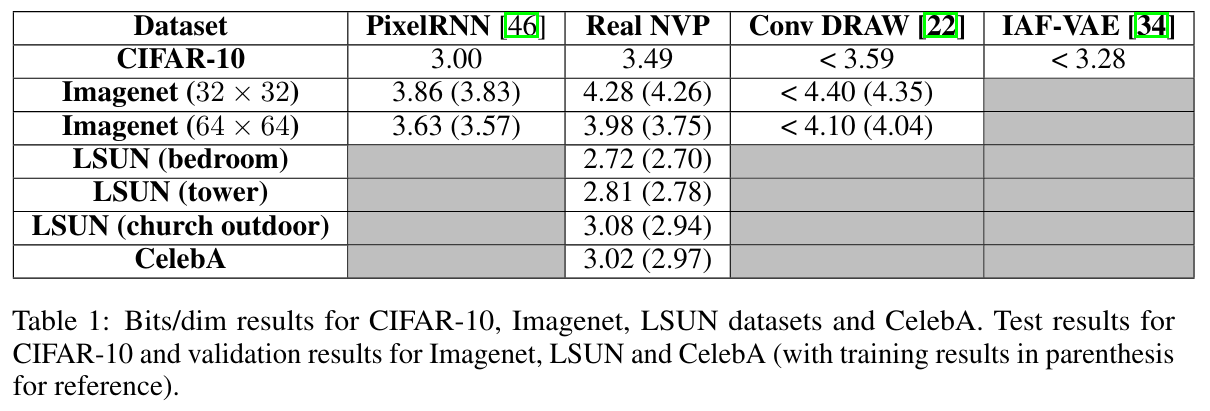
\includegraphics[width=0.8\textwidth]{RealNVPTable.png}
\end{frame}

\begin{frame}
\frametitle{Results: 2}
\center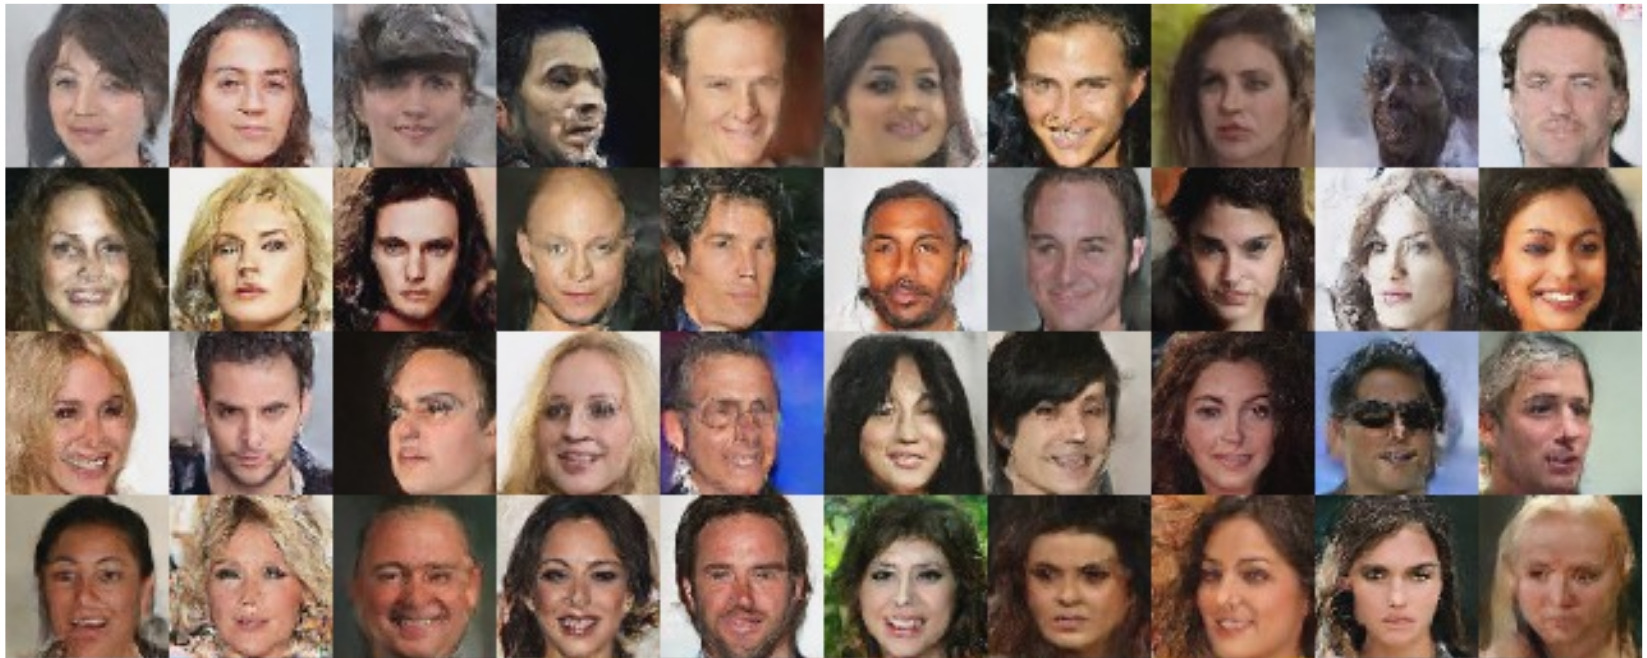
\includegraphics[width=0.8\textwidth]{RealNVPResults.png}
\end{frame}
